\section{Benchmark Examples}

Since the \MA equation became a benchmark problem for fully nonlinear second order PDEs there are same classical test problems for the two-dimensional case. All test cases are solved on the unitsquare $\Omega=[0,1]^2$.

\begin{test} \label{test smooth}
The first classical \MA test is the problem with the data
\[
	u=\exp( \lVert x \rVert_2^2  /2) 
	\text { and } 
	f = (1 + \lVert x \rVert_2^2) \exp( \lVert x \rVert^2).
\]
It has a very smooth solution and is even radial.

\end{test}

\begin{test}\label{test sqrt}
The data
\[
	u = - \sqrt{ 2-  \lVert x \rVert_2^2}
	\text { and } 
	f = 2\left( 2-  \lVert x \rVert_2^2 \right)^{-2}
\]
defines the second example. This test is especially interesting because the convex viscosity solution is only contained in $W^{1,p}(\Omega) $ for $p \in [0,4)$\cite{DG2006a}, i.e. it lacks $H^2$ regularity.
\end{test}

For the next two tests we define $x_0 = \left(\frac 1 2, \frac 1 2  \right)^t$.

\begin{test}\label{test singularity}
The third \MA test is yet more regular. Its solution lies in $C^1$ and it is given by
\[
	u=\frac 1 2 \left( \max 0 {\lVert x - x_0 \rVert_2-0.2 }  \right)^2 
	\text { and } 
	f = \max 0 {1-\frac {0.2} {\lVert x - x_0 \rVert_2} }.
\]
\end{test}


\begin{test}\label{test dirac}
A test determined by
\[
	u = \lVert x - x_0 \rVert_2
	\text { and } 
	f = \pi \delta_{x_0}
\]
describes a cone with origin $x_0$. Note, $f$ is highly non regular. This example does not have a viscosity solution, but $u$ is only an Aleksandrov solution of the problem \cite[Section 2.3.]{FO2011}.
\end{test}


\begin{test}\label{test rhsConst}
A test where the analytical solution is unknown is determined by
\[
	u = 0 \text{ on } \partial \Omega
	\text { and } 
	f = 1
\]
defines the last example.
\end{test}

\section{Numerical Results of a blub}

%read data for case deg=22 and merge into one file
\newcommand{\readDataN}[2]{
\pgfplotstableread{../../FEniCS/data/#1_l2errornorm} #2

\pgfplotstablecreatecol[copy column from table={../../FEniCS/data/#1_h1errornorm}{h1error}] {h1error} #2

\pgfplotstablecreatecol[copy column from table={../../FEniCS/data/#1_newtonSteps}{steps}] {N} #2
}

%\readDataN{MA1_Brenner_deg2}{\MAOneBrennerTwo}
%\readDataN{MA1_Brenner_deg3}{\MAOneBrennerThree}

%\readDataN{MA3_Brenner_deg2}{\MAThreeBrennerTwo}

%\readDataN{MA4_Brenner_deg2}{\MAFourBrennerTwo}
%\readDataN{MA4_Brenner_deg3}{\MAFourBrennerThree}


\readDataN{MA1_Neilan_GradJump_deg22}{\MAOneJumpdegTwoTwo}
\readDataN{MA1_Neilan_GradJump_deg20}{\MAOneJumpdegTwoZero}

\readDataN{MA1_Neilan_deg33}{\MAOnedegThreeThree}
\readDataN{MA1_Neilan_deg32}{\MAOnedegThreeTwo}

%\readDataN{MA2_Neilan_deg22}{\MATwodegTwoTwo}
%\readDataN{MA2_Neilan_deg33}{\MATwodegThreeThree}

%\readDataN{MA3_Neilan_deg22}{\MAThreedegTwoTwo}
%\readDataN{MA3_Neilan_deg33}{\MAThreedegThreeThree}
\readDataN{MA3_Neilan_GradJump_deg22}{\MAThreeJumpdegTwoTwo}
\readDataN{MA3_Neilan_GradJump_deg33}{\MAThreeJumpdegThreeThree}


%\pgfplotstableread{../../FEniCS/data/MA1_Neilan_deg22_l2errornorm} \MAOnedegTwoTwoL
%\pgfplotstableread{../../FEniCS/data/MA1_NeilanGradJump_deg22_l2errornorm} \MAOneJumpdegTwoTwo
%\pgfplotstableread{../../FEniCS/data/MA1_NeilanGradJump_deg22_h1errornorm}\MAOneJumpdegTwoTwoH

%\pgfplotstablecreatecol[copy column from table={../../FEniCS/data/MA1_NeilanGradJump_deg22_h1errornorm}{h1error}] {h1error} \MAOneJumpdegTwoTwo
%\pgfplotstablecreatecol[copy column from table={../../FEniCS/data/MA1_NeilanGradJump_deg22_newtonsteps}{steps}] {N} \MAOneJumpdegTwoTwo


For reference I implemented the algorithm introduced in Section \ref{sec: Brenner method}.
We implemented their presented method using the finite element tool FEniCS \cite{FEniCS}, the Code is append in Appendix. 
To create our initial guess I did not use a vanishing moment method as Brenner suggested, but the solution of $\triangle u = -\sqrt{2f}$ as introduced in \ref{sec: initial guess}. 

I solved the arising nonlinear system of equations with PETSc' basic line search Newton method. 

\begin{table}[h]
	\begin{subtable}[b]{0.45\textwidth}
		\centering
		\pgfplotstabletypeset[columns={iterations, l2error, h1error,N},
				    every row 0 column 0/.style={set content=init},
		]\MAOneBrennerTwo
    	\caption{Error for $k=2$}
   \end{subtable}
   ~
	\begin{subtable}[b]{0.45\textwidth}
		\centering
		\pgfplotstabletypeset[columns={iterations, l2error, h1error,N},
				    every row 0 column 0/.style={set content=init},
		]\MAOneBrennerThree
 	\caption{Error for $k=3$}
	\end{subtable}
	\caption{Errors for test case \ref{test smooth}}
	\label{tab: l2 errors test 1 Brenner}
\end{table}


\begin{figure}[h!]
\centering
	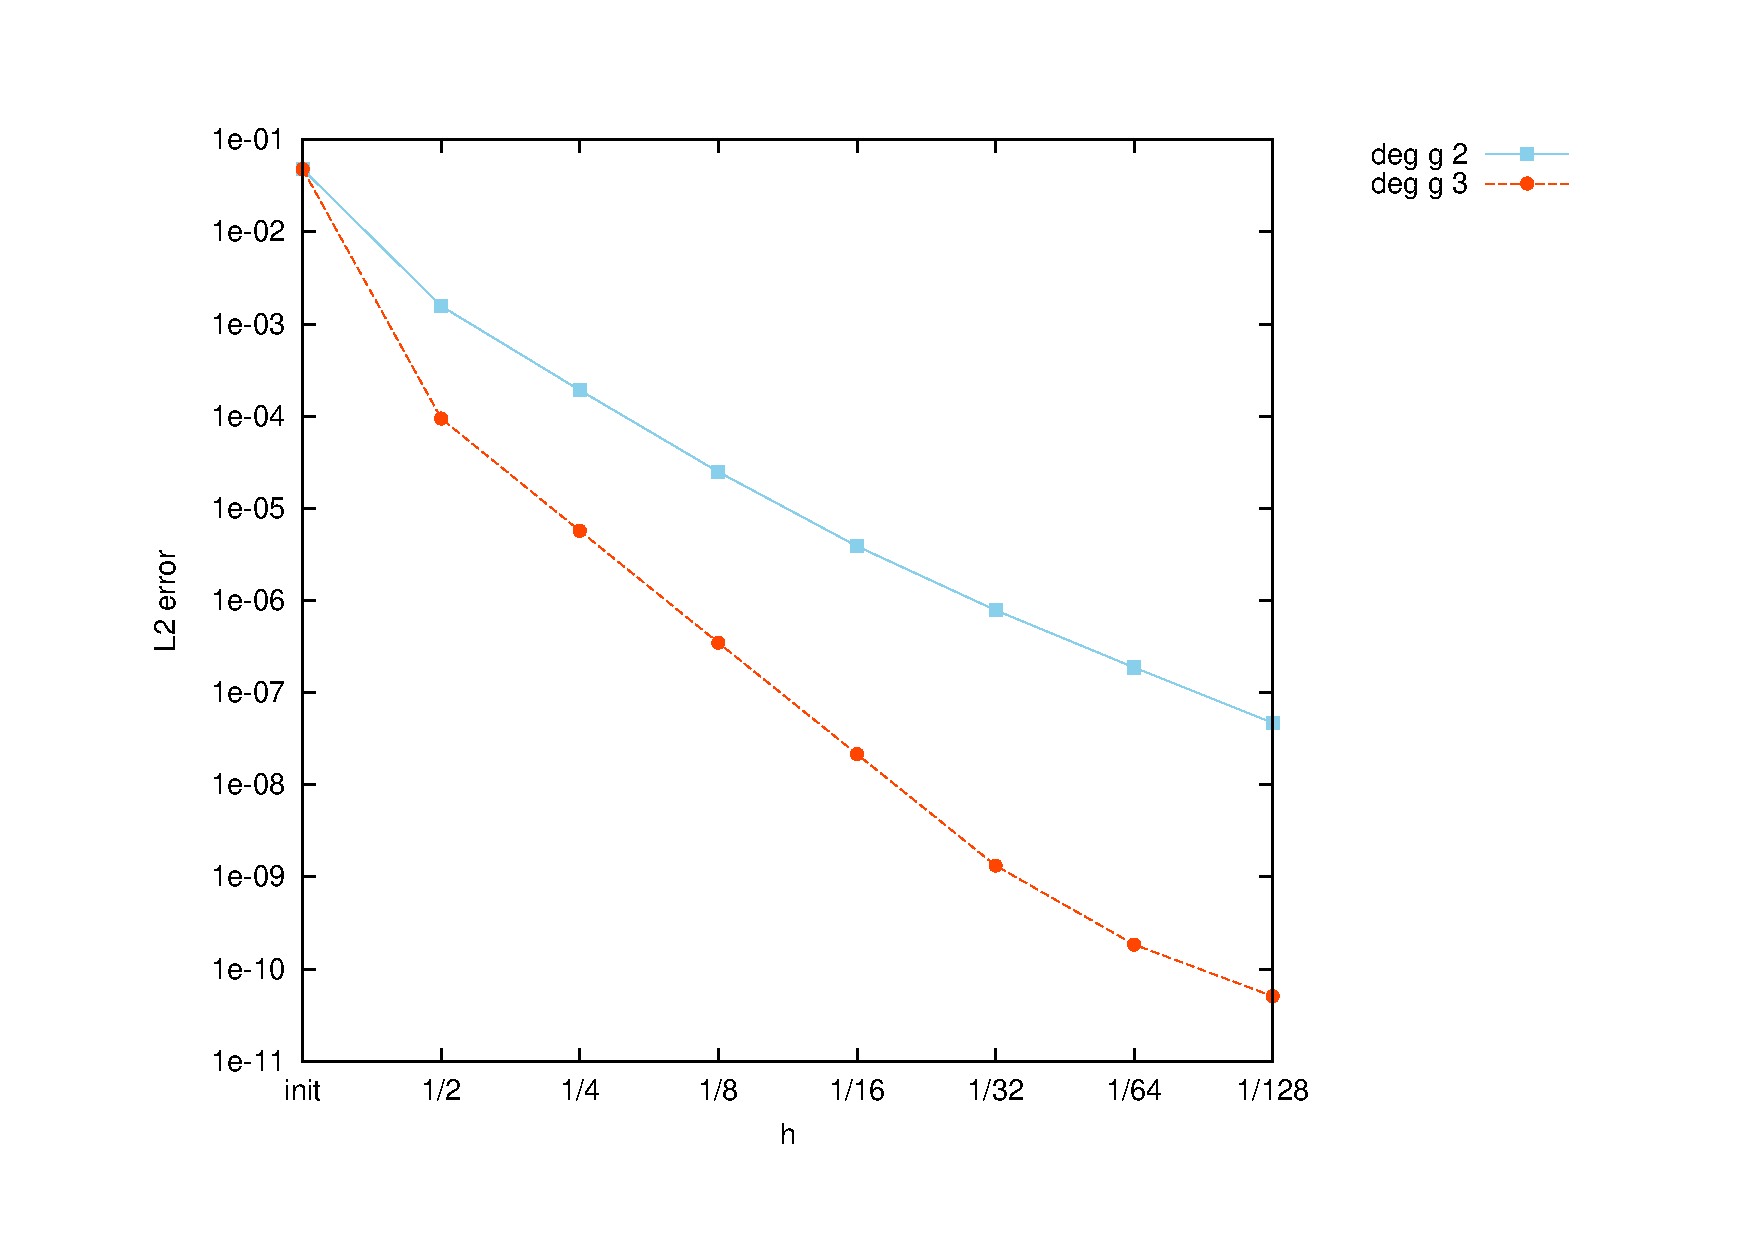
\includegraphics[scale=0.4]{../../FEniCS/diagrams/MA1_Brenner_l2.pdf}
	\caption{$L^2$ errors for test case \ref{test smooth}}
\end{figure}

For the second test case the Newton did not even on the coarsest grid converge. Also in the third test case our Newton solver had problems. You can see results of the runs for $h=1/2, \dots, 1/16$ in table \ref{tab: l2 errors test 3 Brenner}, for finer grid the solver did not converge. My attempts to solve this example with FEniCS' built in damped Newton method with different relaxation parameters did also not succeed on any grid finer than $1/16$.
\begin{table}[h]
		\centering
		\pgfplotstabletypeset[columns={iterations, l2error, h1error,N},
				    every row 0 column 0/.style={set content=init},
		]\MAThreeBrennerTwo
    	\caption{Error for $k=2$}
	\caption{Errors for test case \ref{test singularity}}
	\label{tab: l2 errors test 3 Brenner}
\end{table}

The fourth example does not have not a classical solution. As in the previous cases the method does not converge and after some steps the Newton solver does not converge on the provided initial guesses. The corresponding results are shown in table \ref{tab: l2 errors test 4 Brenner}.

\begin{table}[h]
	\begin{subtable}[b]{0.45\textwidth}
		\centering
		\pgfplotstabletypeset[columns={iterations, l2error, h1error,N},
				    every row 0 column 0/.style={set content=init},
				    columns/l2error/.style={ /pgf/number format/sci precision=6}     % print 14 digits
		]\MAFourBrennerTwo
    	\caption{Error for $k=2$}
   \end{subtable}
   ~
	\begin{subtable}[b]{0.45\textwidth}
		\centering
		\pgfplotstabletypeset[columns={iterations, l2error, h1error,N},
				    every row 0 column 0/.style={set content=init},
		]\MAFourBrennerThree
 	\caption{Error for $k=3$}
	\end{subtable}
	\caption{Errors for test case \ref{test dirac}}
	\label{tab: l2 errors test 4 Brenner}
\end{table}

\newpage
\section{Numerical Results of a Finite Element Method based on a Disrete Hessian}

I also implemented the algorithm introduced in Section \ref{sec: FEM discrete Hessian}.
Additional to the numerical results Neilan presented it is interesting to explore what happens if we vary the polynomial degree for the Hessian ansatz space. 

The implementation was also done with the Finite Element Tool FEniCS \cite{FEniCS}. The uniform triangulation $\triang$ was obtained by first dividing the domain into squares of side length $h$ and then split them into 4 triangles by drawing both diagonals. \\
Different to the initial guess suggested in \cite{Neilan2014} I used the solution of $\triangle u = -\sqrt{2f}$ as introduced in \ref{sec: initial guess}. 
We denote the degree of the trial space $V_h=P_h^k \cap H^1(\Omega)$ by $k$ and the degree chosen for the Hessian ansatz space $\Sigma_h = [\mathcal{P}_h^{k_{DH}}]^{d \times d}$ by $k_{DH}$. The nonlinear system of equations given by \eqref{eq: neilan eq1} and \eqref{eq: discrete hessian} or \eqref{eq: neilan eq1 + jump} and \eqref{eq: discrete hessian}, respectively was solved with PETSc' basic line search Newton method. 
%SNES Object: 1 MPI processes
%  type: newtonls
%  SNES has not been set up so information may be incomplete
 % maximum iterations=10, maximum function evaluations=2000
 % tolerances: relative=1e-09, absolute=1e-08, solution=1e-16
  %total number of linear solver iterations=0
  %total number of function evaluations=0
  %SNESLineSearch Object:   1 MPI processes
   % type: bt
    %  interpolation: cubic
   %   alpha=1.000000e-04
  %  maxstep=1.000000e+08, minlambda=1.000000e-12
 %   tolerances: relative=1.000000e-08, absolute=1.000000e-15, lambda=1.000000e-08
  %  maximum iterations=40
  %KSP Object:   1 MPI processes
    %type: preonly
    %maximum iterations=10000, initial guess is zero
   % tolerances:  relative=1e-05, absolute=1e-50, divergence=10000
   % left preconditioning
   % using DEFAULT norm type for convergence test
  %PC Object:   1 MPI processes
  %  type: lu
  %  PC has not been set up so information may be incomplete
    %  LU: out-of-place factorization
   %   tolerance for zero pivot 2.22045e-14
   %   matrix ordering: nd
   % linear system matrix = precond matrix:
   % Matrix Object:     1 MPI processes
    %  type: seqaij
    %  rows=112, cols=112
    %  total: nonzeros=2744, allocated nonzeros=2744
    %  total number of mallocs used during MatSetValues calls =0
      %  using I-node routines: found 80 nodes, limit used is 5

Most parameters were set to the default PETSc values %which includes the solver uses cubic backtracking 
but the absolute tolerance was adjusted to $1e-8$ and the number of maximum iteration was restricted to 50. 

Figure \ref{fig: l2 errors test 1} shows the $L^2$ error of all performances of the first test case that have converged, the polynomial degrees $k$ were taken to be $1,\dots,3$ and $k_{DH}$ equal to all variants $0, \dots, k$.  The results for the runs with $k=3$ are shown more detailed in Table \ref{tab: l2 errors test 1 deg 2}, in both tables the column $N$ refers to the number of iterations the Newton solver needed to reach the desired tolerance. 

\begin{figure}[h!]
\centering
	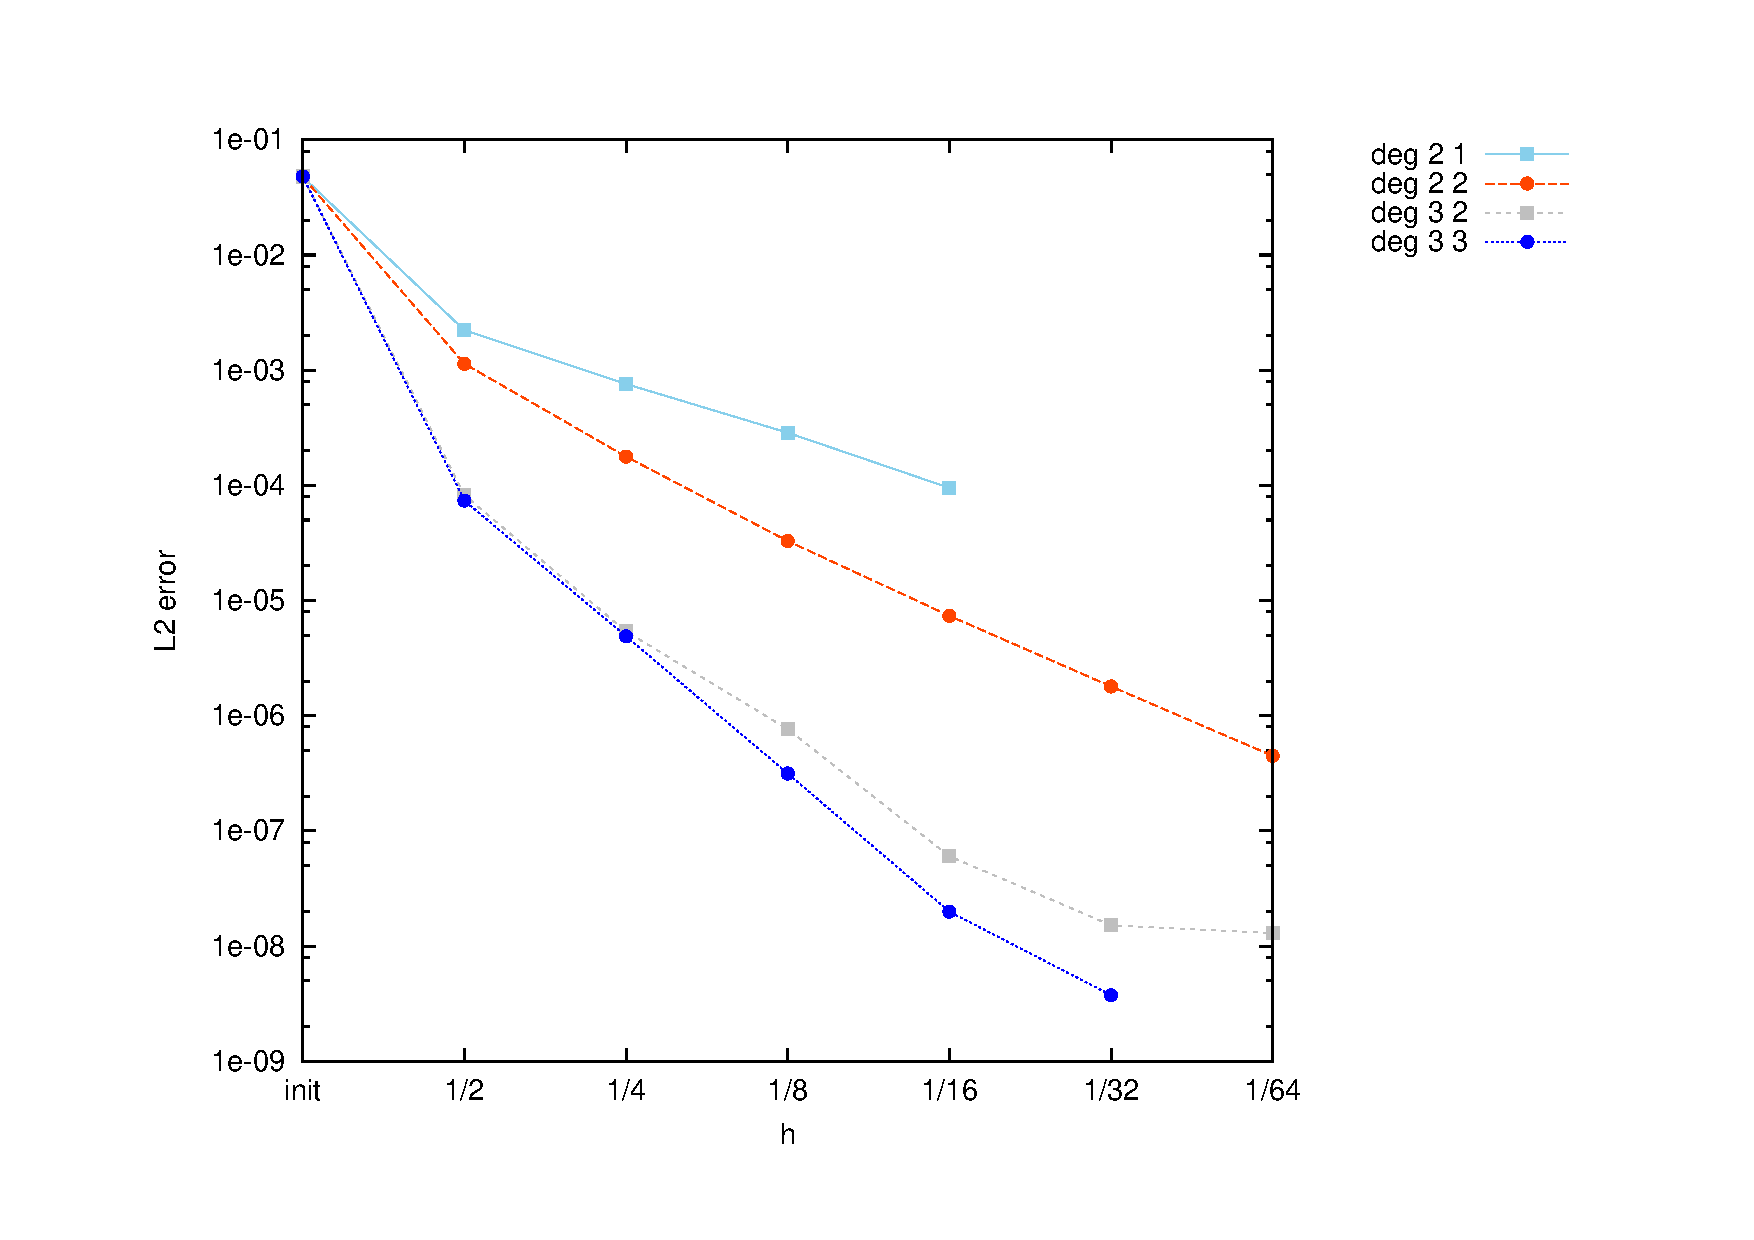
\includegraphics[scale =0.4]{../../FEniCS/diagrams/MA1_Neilan_l2.pdf}
	\caption{$L^2$ errors for test case \ref{test smooth}}
	\label{fig: l2 errors test 1}
\end{figure}
 \todo{memory errors}
 Unfortunately the calculation for $k=3$ could not be carried out since 
 0]PETSC ERROR: Out of memory. This could be due to allocating
 [0]PETSC ERROR: too large an object or bleeding by not properly
 [0]PETSC ERROR: destroying unneeded objects.
 [0]PETSC ERROR: Memory allocated 0 Memory used by process 15882436608
 PETSC ERROR: Try running with -malloc\_dump or -malloc\_log for info.
 PETSC ERROR: Memory requested 18446744065119617024!
 
\begin{figure}[h!]
\centering
	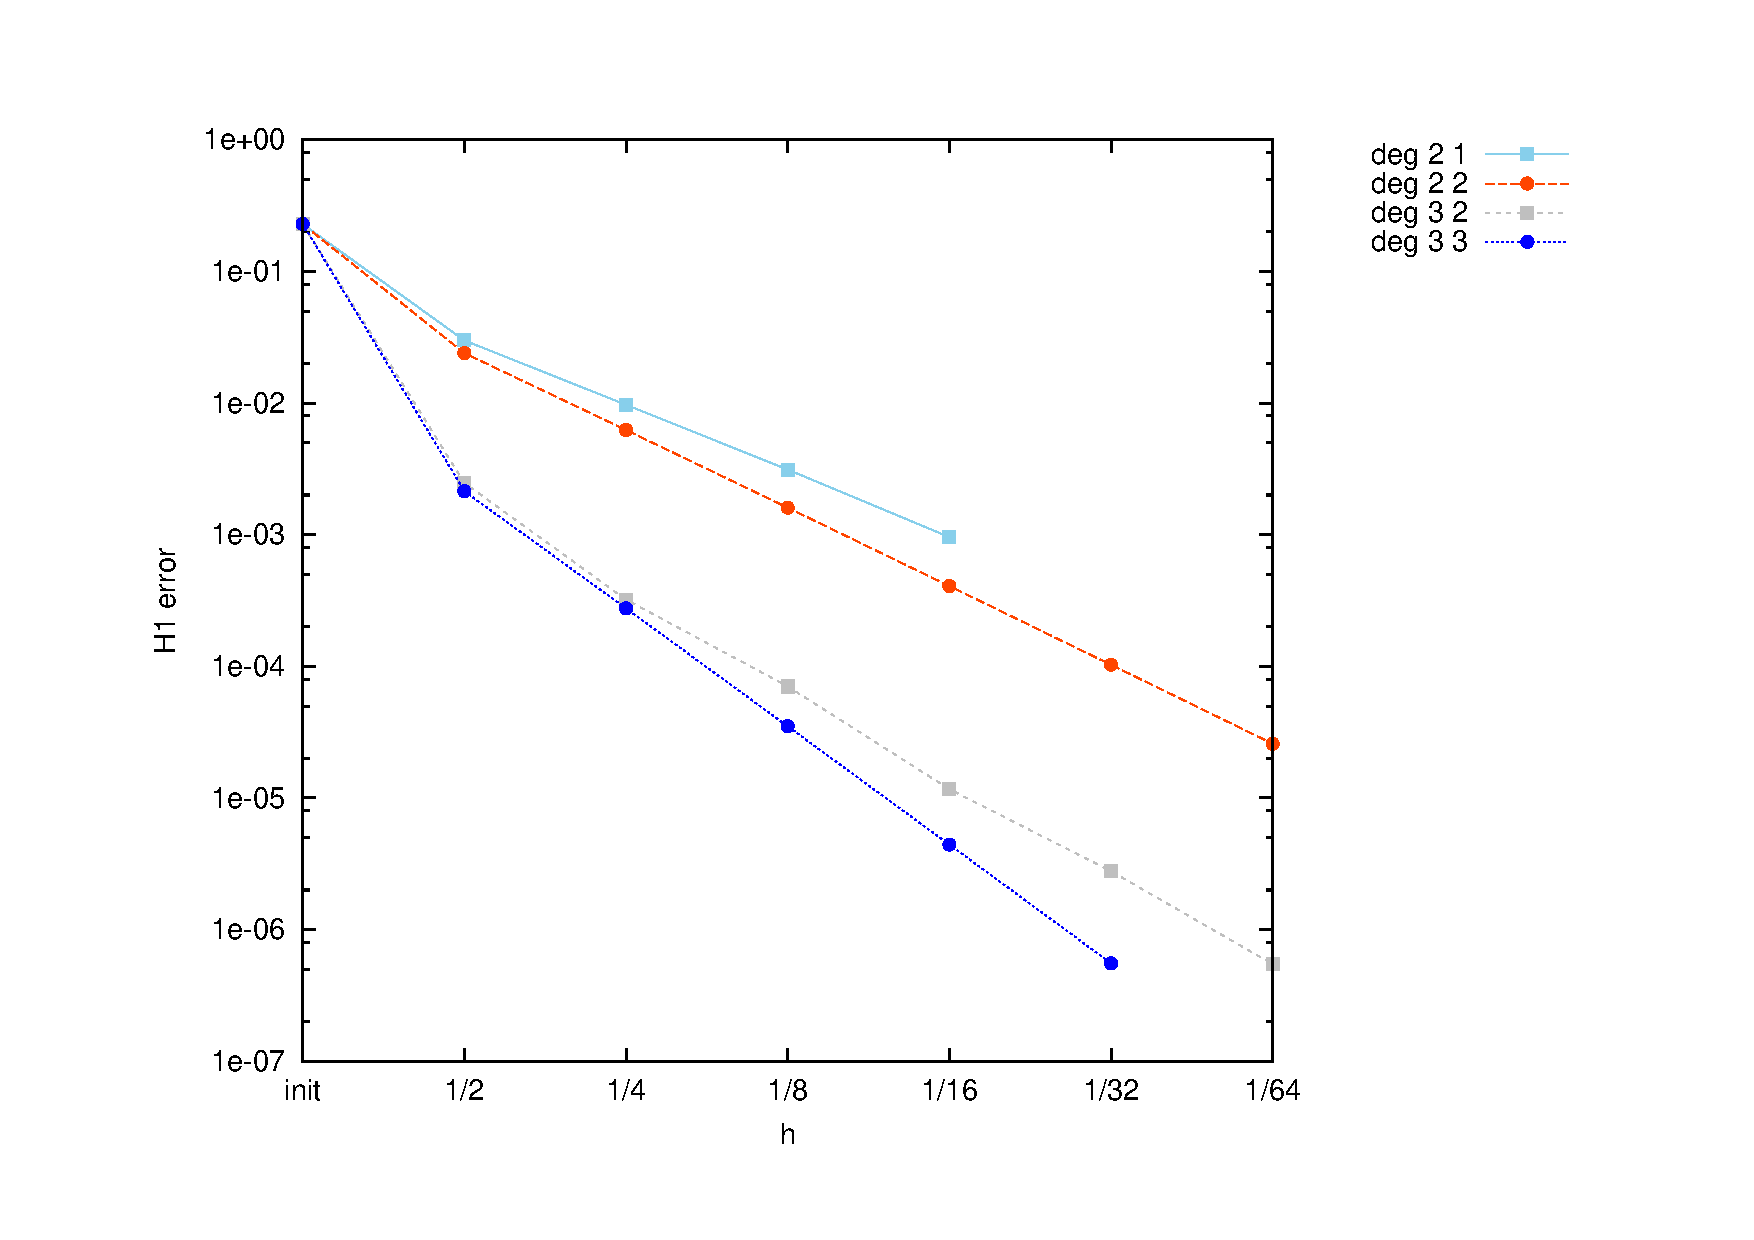
\includegraphics[scale =0.4]{../../FEniCS/diagrams/MA1_Neilan_h1.pdf}
	\caption{$H^1$ errors for test case \ref{test smooth}}
	\label{fig: h2 errors test 1}
\end{figure}

\begin{table}[h]
	\begin{subtable}[b]{0.45\textwidth}
		\centering
		\pgfplotstabletypeset[columns={iterations, l2error, h1error,N},
				    every row 0 column 0/.style={set content=init},
		]\MAOnedegThreeThree
    	\caption{Error for $k=3, k_{DH}=3$}
   \end{subtable}
   ~
	\begin{subtable}[b]{0.45\textwidth}
		\centering
		\pgfplotstabletypeset[columns={iterations, l2error, h1error,N},
				    every row 0 column 0/.style={set content=init},
		]\MAOnedegThreeTwo
 	\caption{Error for $k=3, k_{DH}=2$}
	\end{subtable}
	\caption{Errors for test case \ref{test smooth}}
	\label{tab: l2 errors test 1 deg 2}
\end{table}


Considering the results of the smooth test scenario we notice that the error almost do not alter for different polynomial degrees $k_{DH}$ if both converge. Albeit it seems for low polynomial degrees a difference between those degrees leads to divergence.

This test scenario was also performed with the additional normal jump penalty term as stated in \eqref{eq: neilan eq1 + jump} weighted with $\eta$ equal to 50 leading to the results shown in figure \ref{fig: l2 errors test 1 jump} and the tables \ref{tab: l2 errors test 1 deg 2 jump}.

\begin{figure}[h!]
\centering
	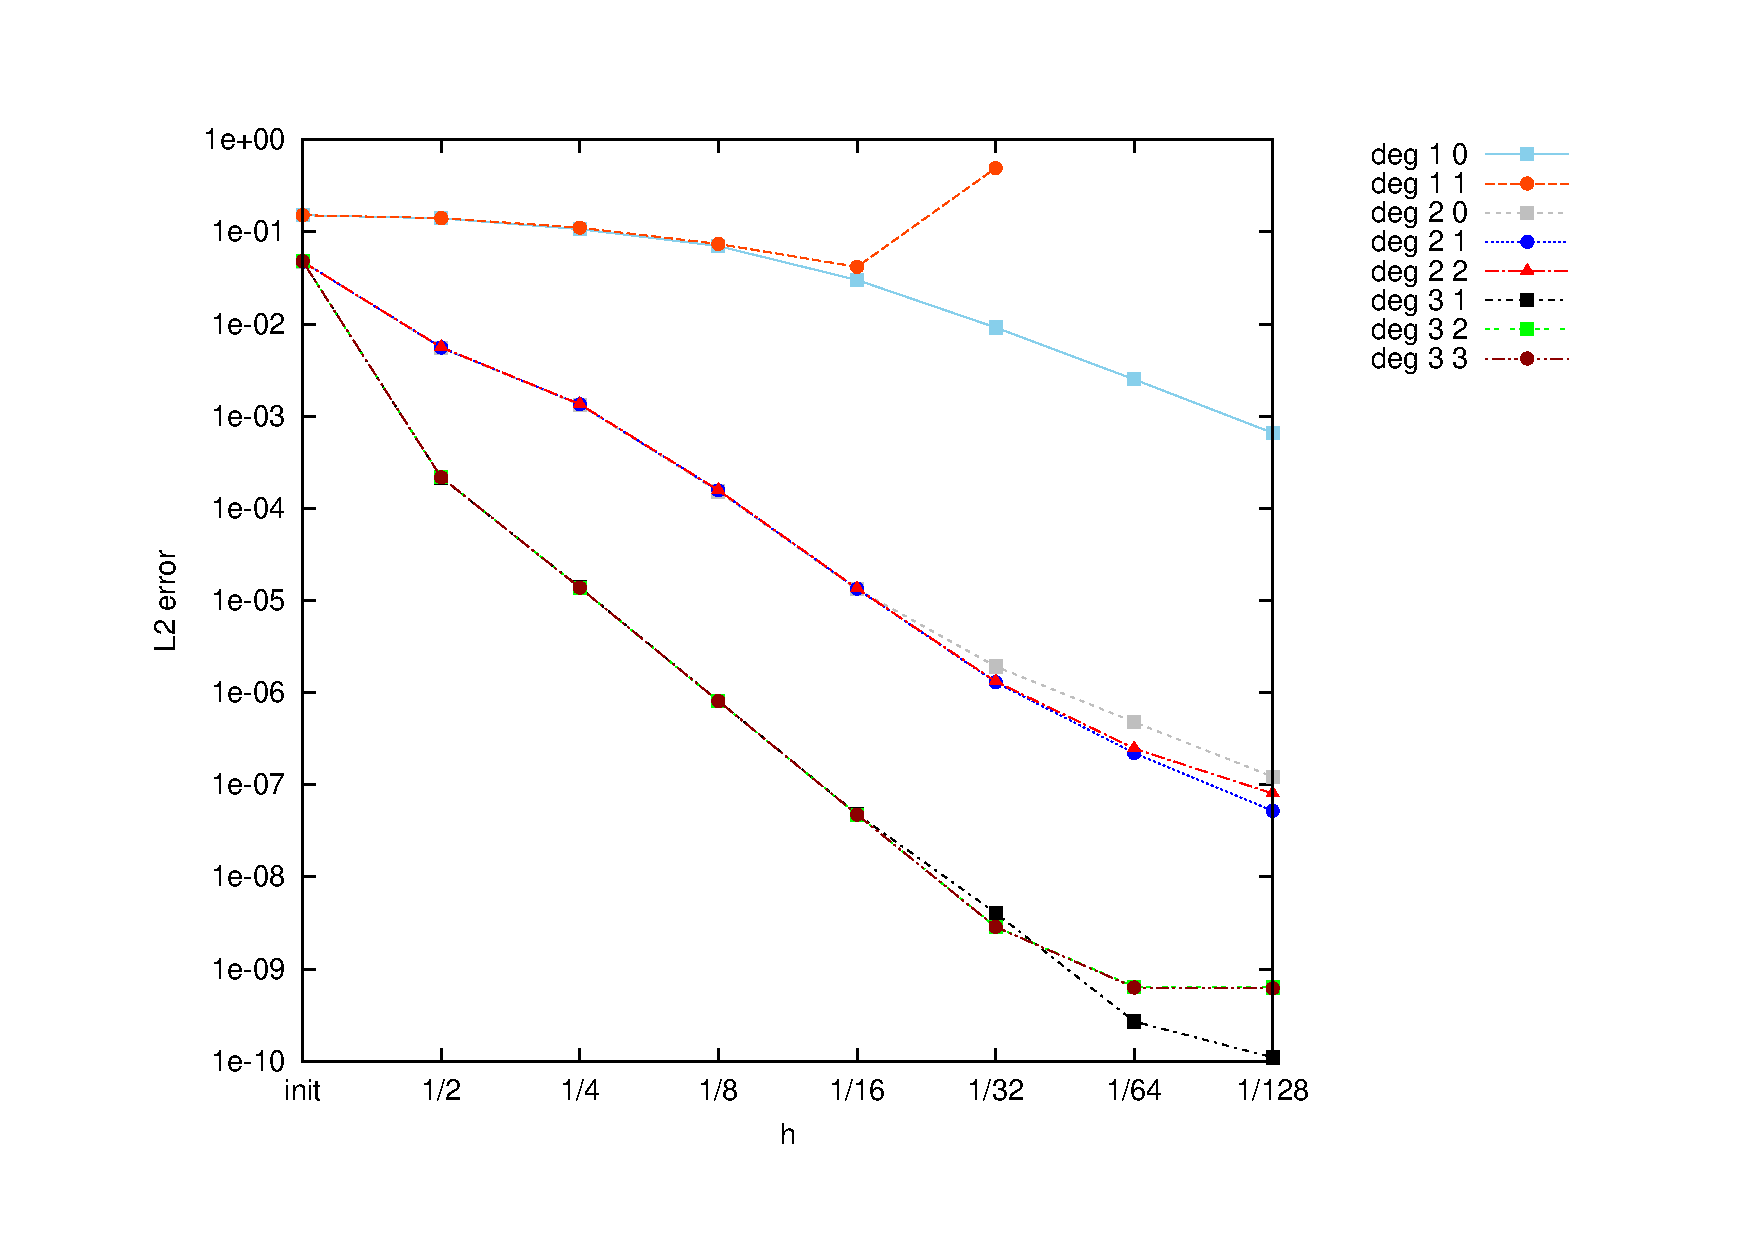
\includegraphics[scale=0.4]{../../FEniCS/diagrams/MA1_Neilan_GradJump_l2.pdf}
	\caption{$L^2$ errors for test case \ref{test smooth} and additional gradient jump penalty}
	\label{fig: l2 errors test 1 jump}
\end{figure}

\begin{figure}[h!]
\centering
	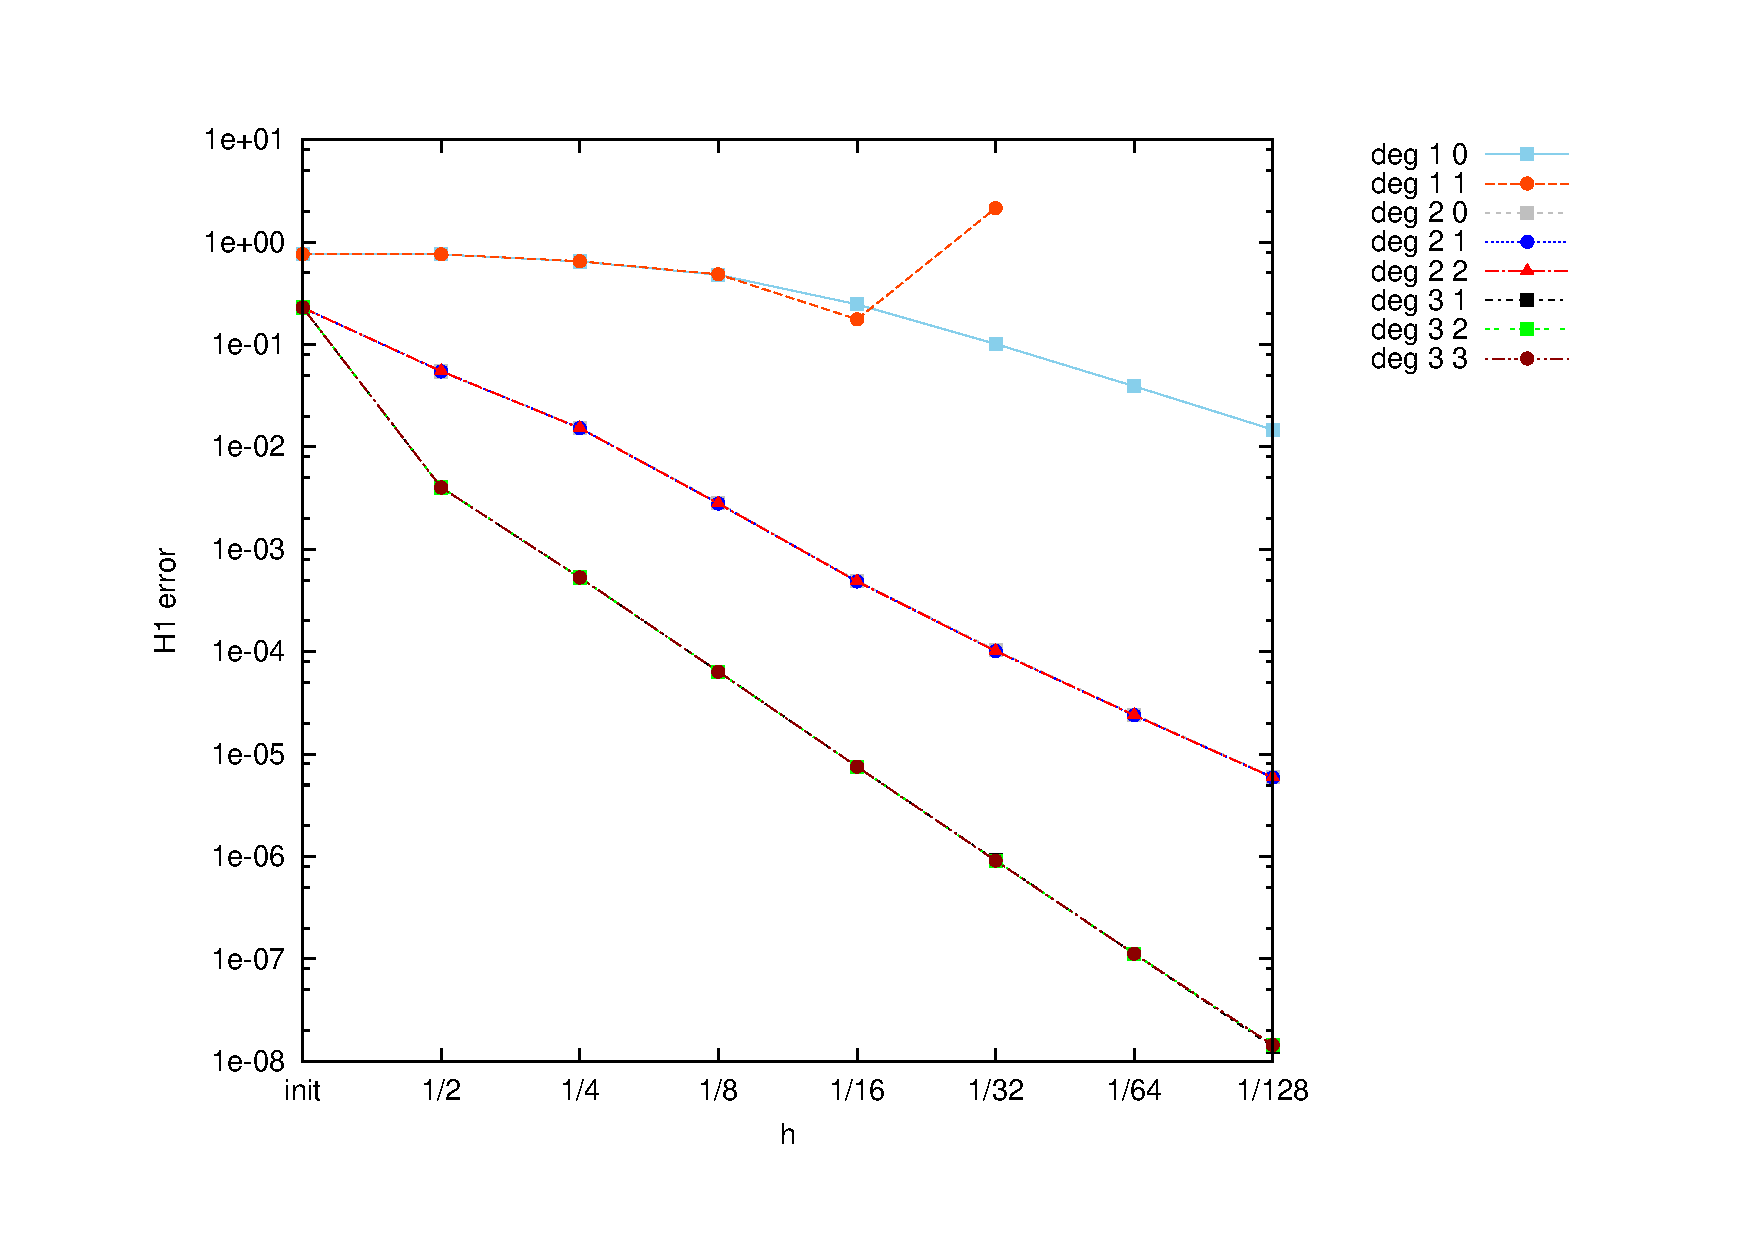
\includegraphics[scale =0.4]{../../FEniCS/diagrams/MA1_Neilan_GradJump_h1.pdf}
	\caption{$H^1$ errors for test case \ref{test smooth} and additional gradient jump penalty}
	\label{fig: h1 errors test 1 jump}
\end{figure}

\begin{table}[h]
	\begin{subtable}[b]{0.45\textwidth}
		\centering
		\pgfplotstabletypeset[
		columns={iterations, l2error, h1error,N},
		    every row 0 column 0/.style={set content=init},
		]\MAOneJumpdegTwoTwo
    	\caption{Error for $k=2, k_{DH}=2$}
   \end{subtable}
   ~
	\begin{subtable}[b]{0.45\textwidth}
		\centering
		\pgfplotstabletypeset[columns={iterations, l2error, h1error,N},
		    every row 0 column 0/.style={set content=init},
		]\MAOneJumpdegTwoZero
	\caption{Error for $k=2, k_{DH}=0$}
	\end{subtable}
	\caption{Errors for test case \ref{test smooth}}
	\label{tab: l2 errors test 1 deg 2 jump}
\end{table}

\todo{Kommentar zu diesen Ergebnissen.}

\begin{table}
	\pgfplotstabletypeset
	{
		k $k_{DH}$ {numerical order}
		1 0 0.873103
		2 0 2.35083
		2 1 2.29612
		2 2 2.37389
		3 1 3.83759
		3 2 3.33588
		3 3 3.33706
	}
\caption{order calculated fitted the data for the case with a jump penalty}
\label{tab: order jump}
\end{table}


The test two was carried out for $\eta=20k^2$


\newpage

\section{Numerical Results of Our DG Method}

Our method was implemented in pure C++. The underlying grid structure was taken from the implementation of \cite{BMV2009}, handling vectors and matrices as well as was linear solver were provided by the Eigen library \cite{eigenweb}. To solve the quadratic program arising in the context of convexification the C++ library ipopt \cite{ipopt} was used.

For a initial guess I also used the solution of $\triangle u = -\sqrt{2f}$ combined with the multilevel approach as described in \ref{sec: initial guess}.
The arising linear system of equations was solved with Eigen's internal Cholesky solver.
The parameters were if not other specified taken to be $\sigma=10 k^2, \sigma_G = 50, \alpha =
0.3$ and $\varepsilon = 1e-2$.
In the first figure \ref{fig: l2 errors test 1 ourMethod} there were carried out 15 steps before a further refinement.

\begin{figure}[h!]
	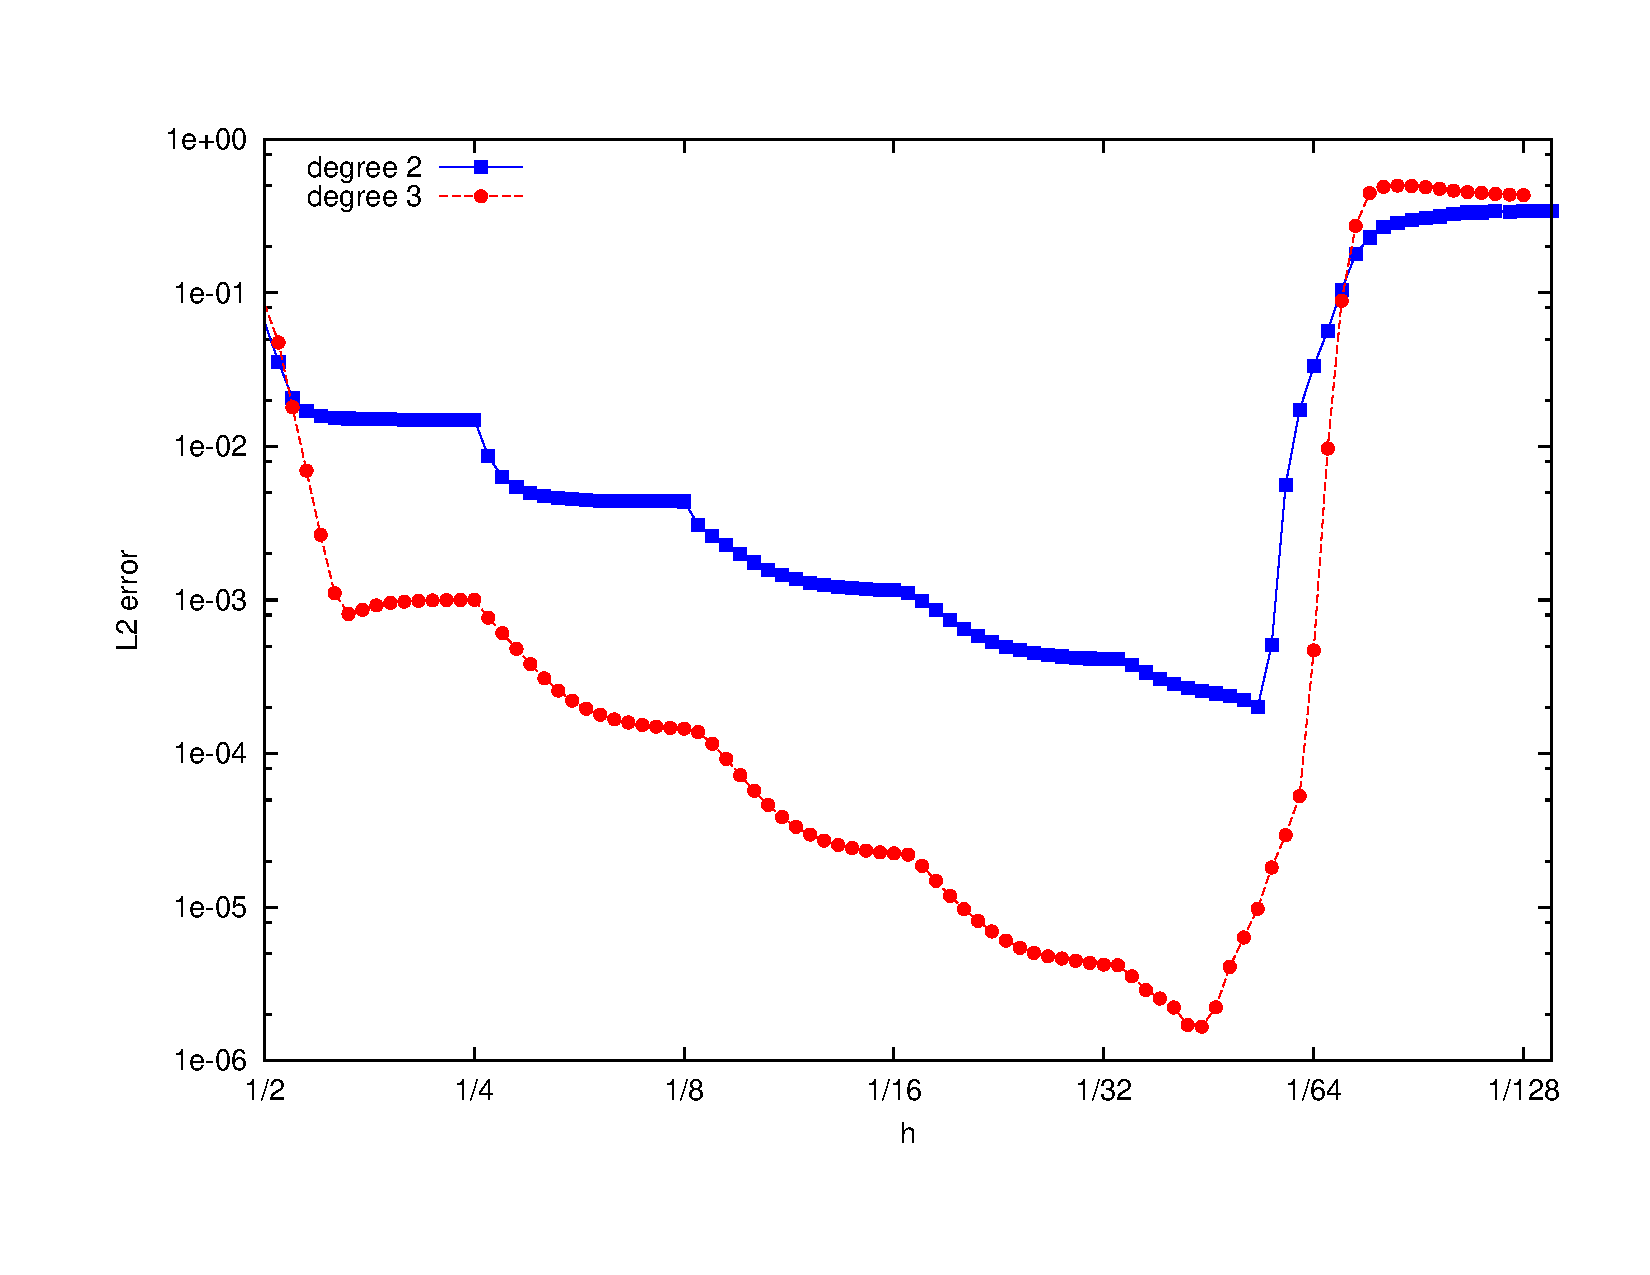
\includegraphics[scale =0.5]{plots/MA1.pdf}
	\caption{Relative $L^2$ errors for test case \ref{test smooth} and additional gradient jump penalty}
	\label{fig: l2 errors test smooth ourMethod}
\end{figure}

\begin{figure}[h!]
	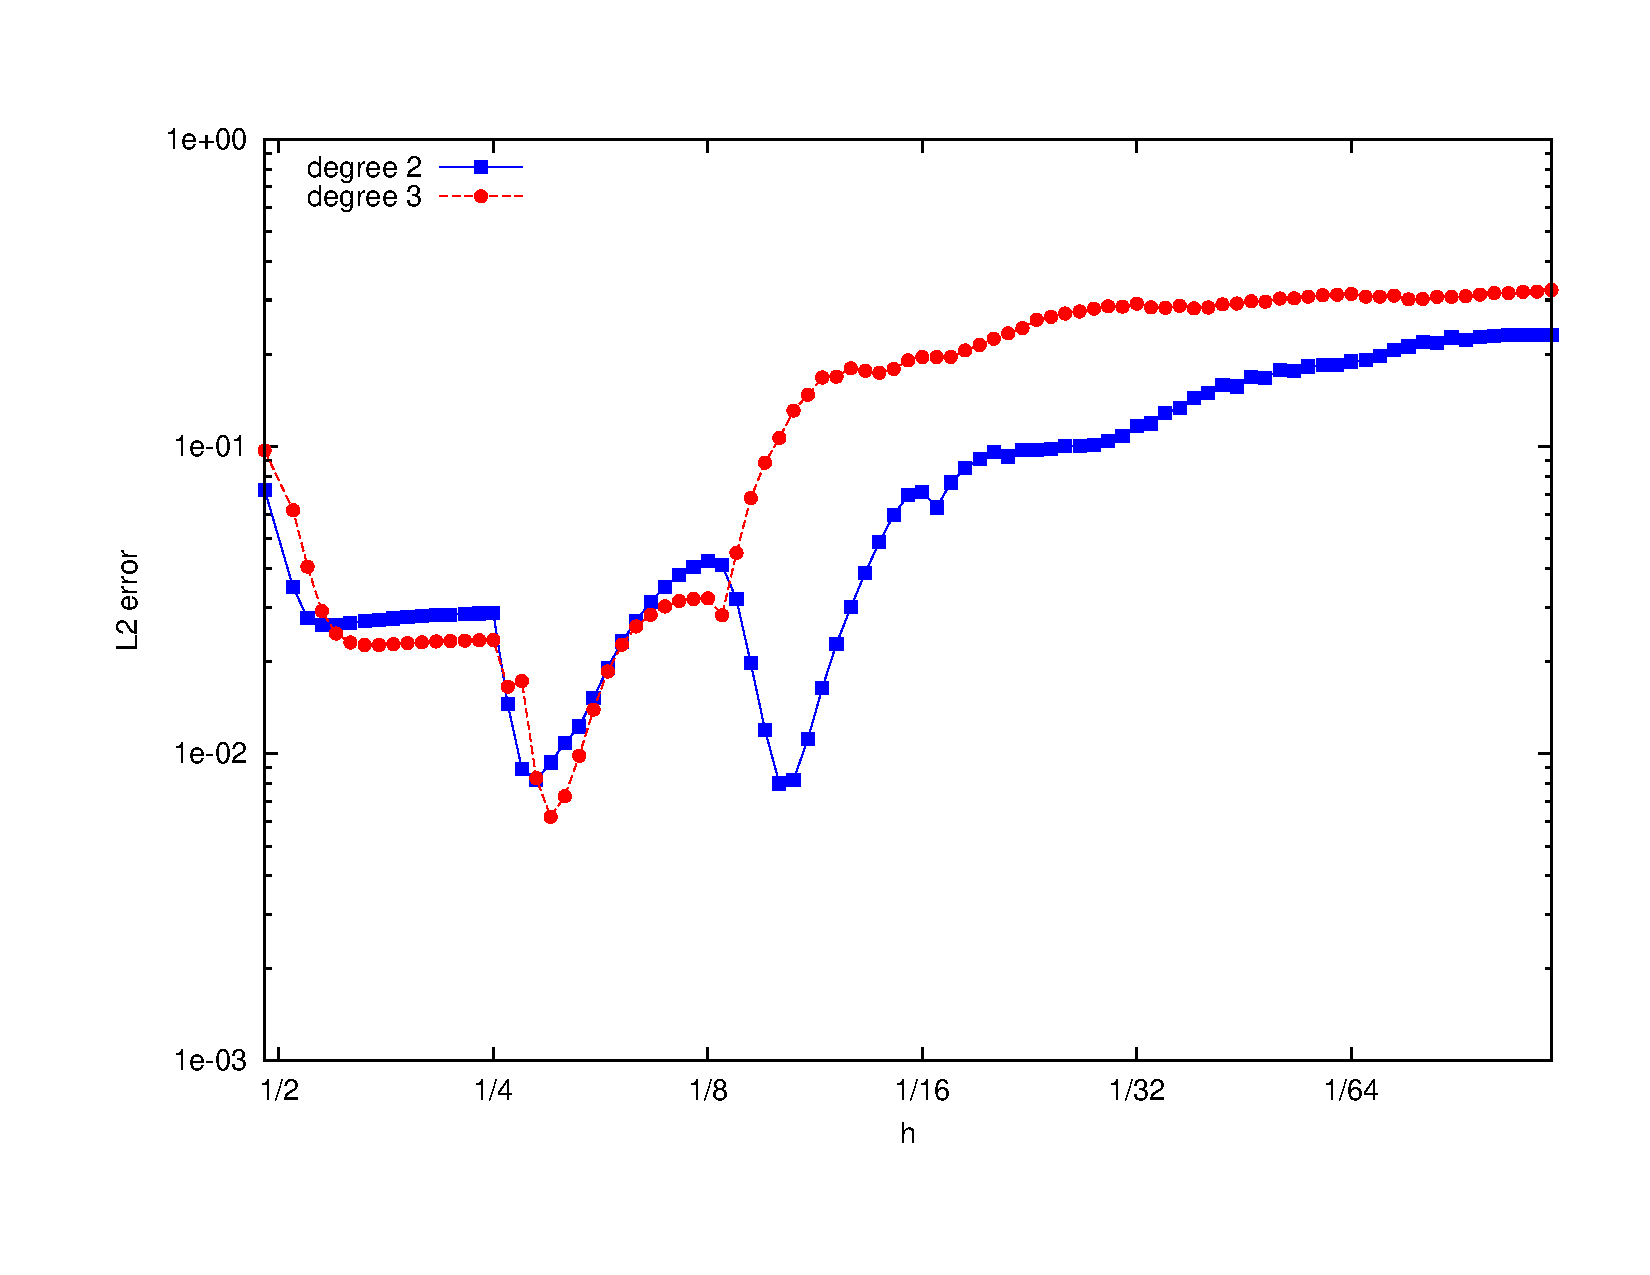
\includegraphics[scale =0.5]{plots/MA3.pdf}
	\caption{$L^2$ errors for test case \ref{test sqrt} and additional gradient jump penalty}
	\label{fig: l2 errors test sqrt ourMethod}
\end{figure}


\begin{figure}[h!]
	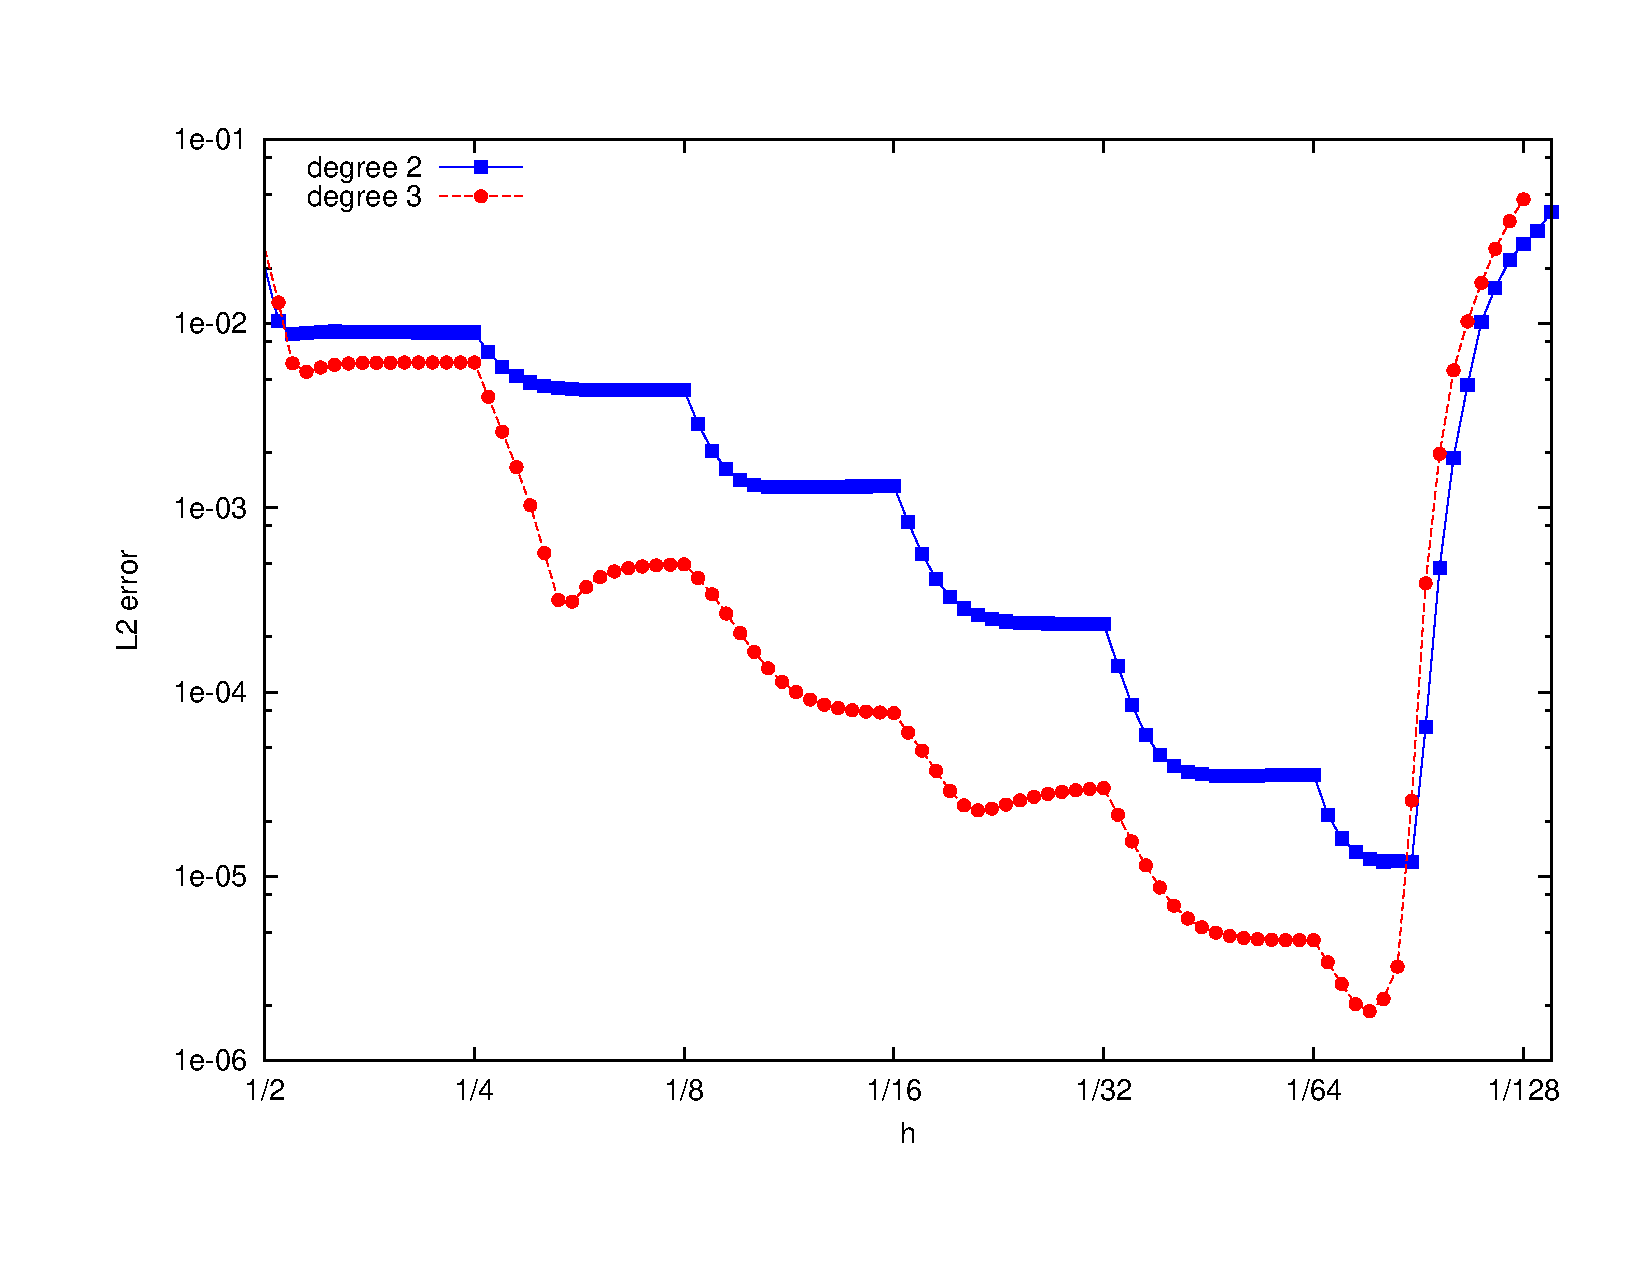
\includegraphics[scale =0.5]{plots/MA2.pdf}
	\caption{$L^2$ errors for test case \ref{test singularity} and additional gradient jump penalty}
	\label{fig: l2 errors test singularity ourMethod}
\end{figure}



?????
While Awanou uses a finite difference scheme to solve the PDE in every step we want to exploit the benefits of a DG method and solve every intermediate step by a SIPG method. 
